\samerowans{\begin{problem}{1}
$KE$ --- биссектриса $\angle{CKB}$, $\angle{AKD} = 40^{\text{o}}$, $DK \perp CK$. Найдите $\angle{CKE}$.
\end{problem}} 

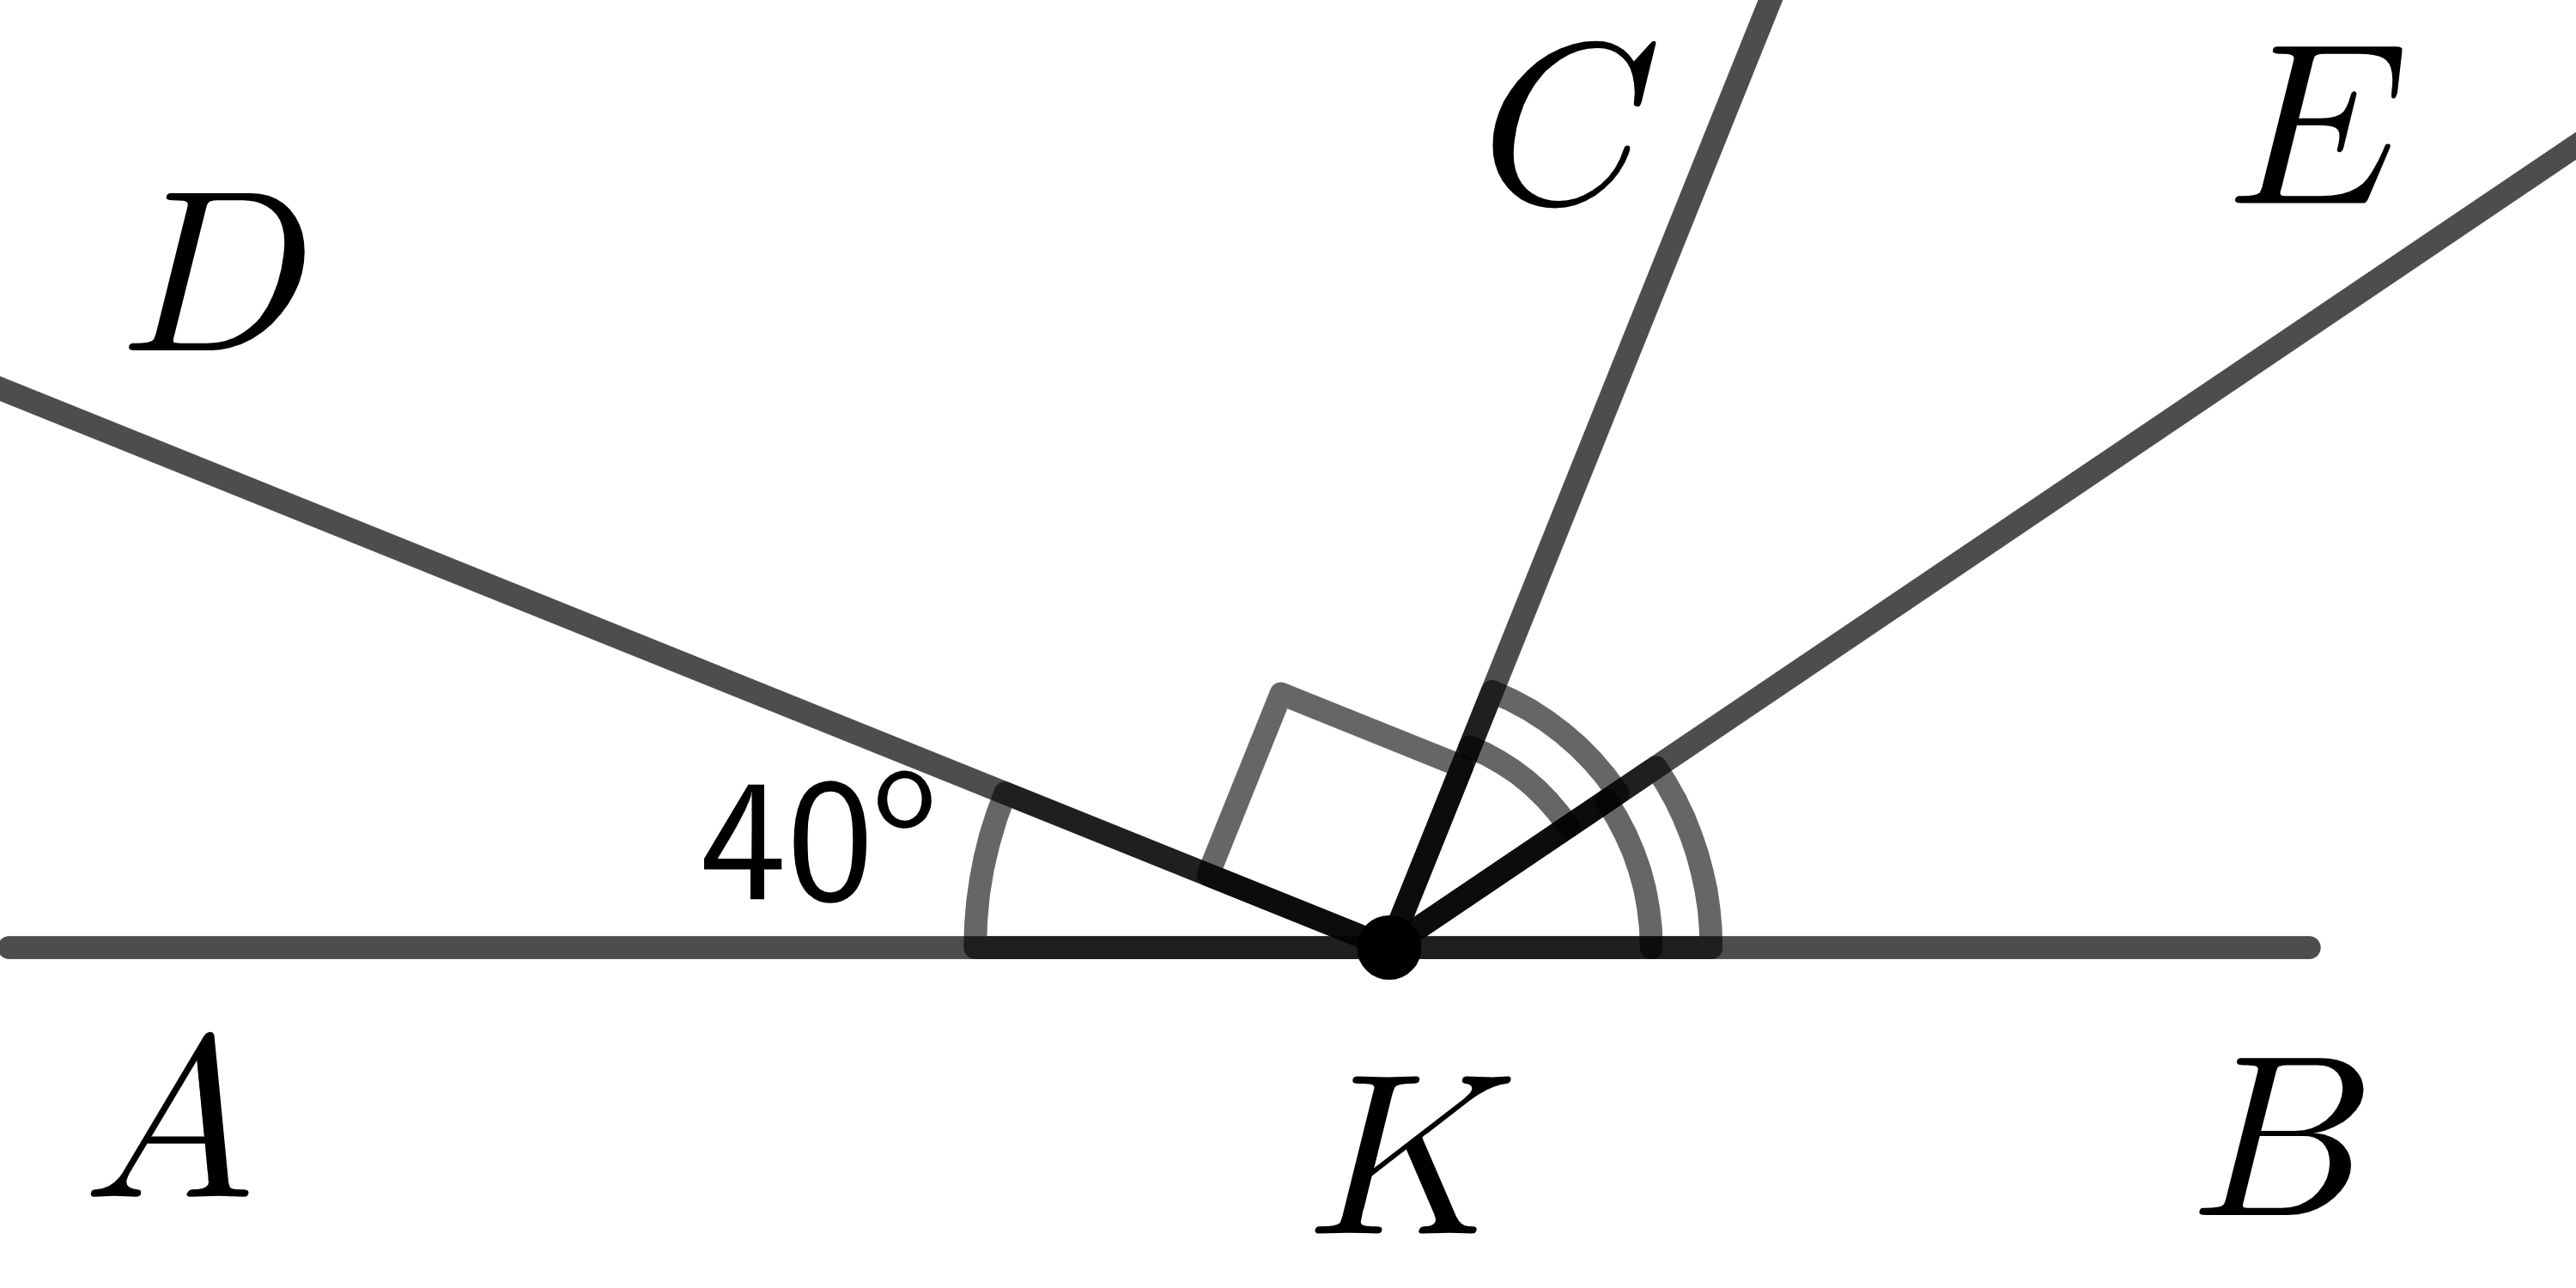
\includegraphics[width=.3\textwidth]{20260404/pics/20260404_geom_for_mat_01_v2.png}

\samerowans{\begin{problem}{2a}
Прямые $a$ и $b$ параллельны. По данным чертежа найдите неизвестные углы $x$, $y$ и $z$.
\end{problem}} 

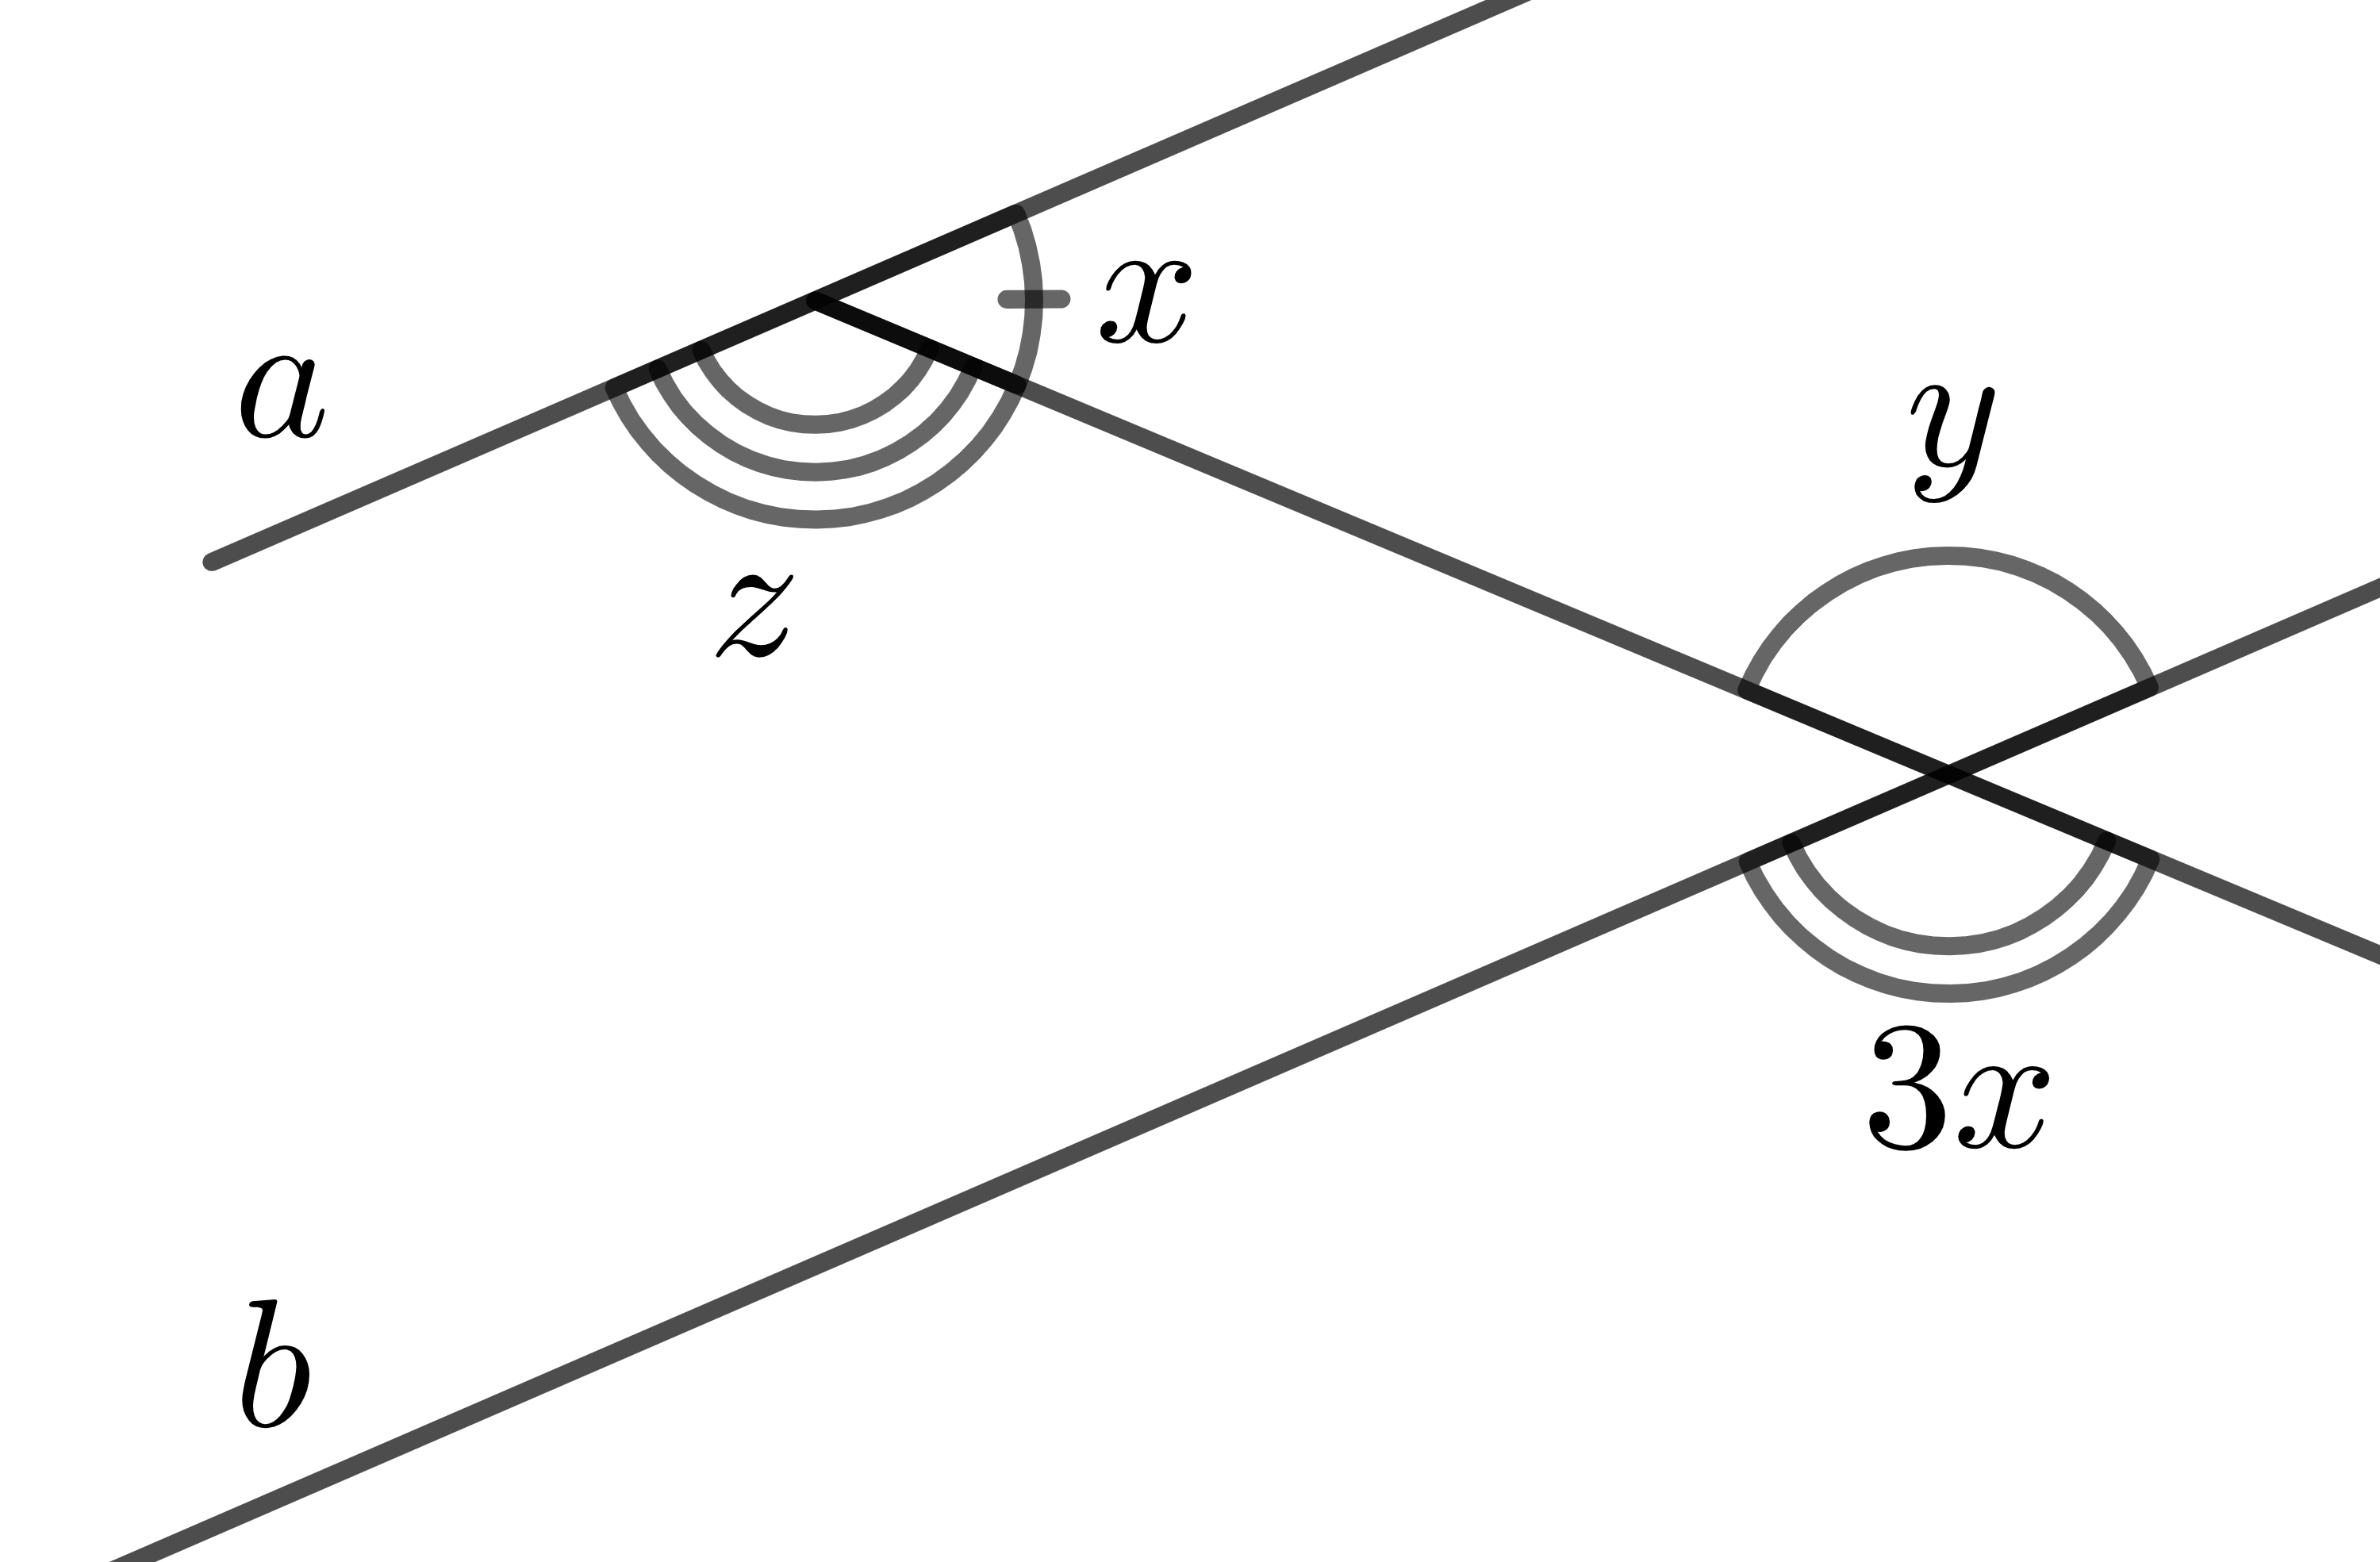
\includegraphics[width=.3\textwidth]{20260404/pics/20260404_geom_for_mat_02a_v2.png}

\samerowans{\begin{problem}{2b}
Прямые $a$ и $b$ параллельны. По данным чертежа найдите неизвестные углы $x$, $y$ и $z$.
\end{problem}} 

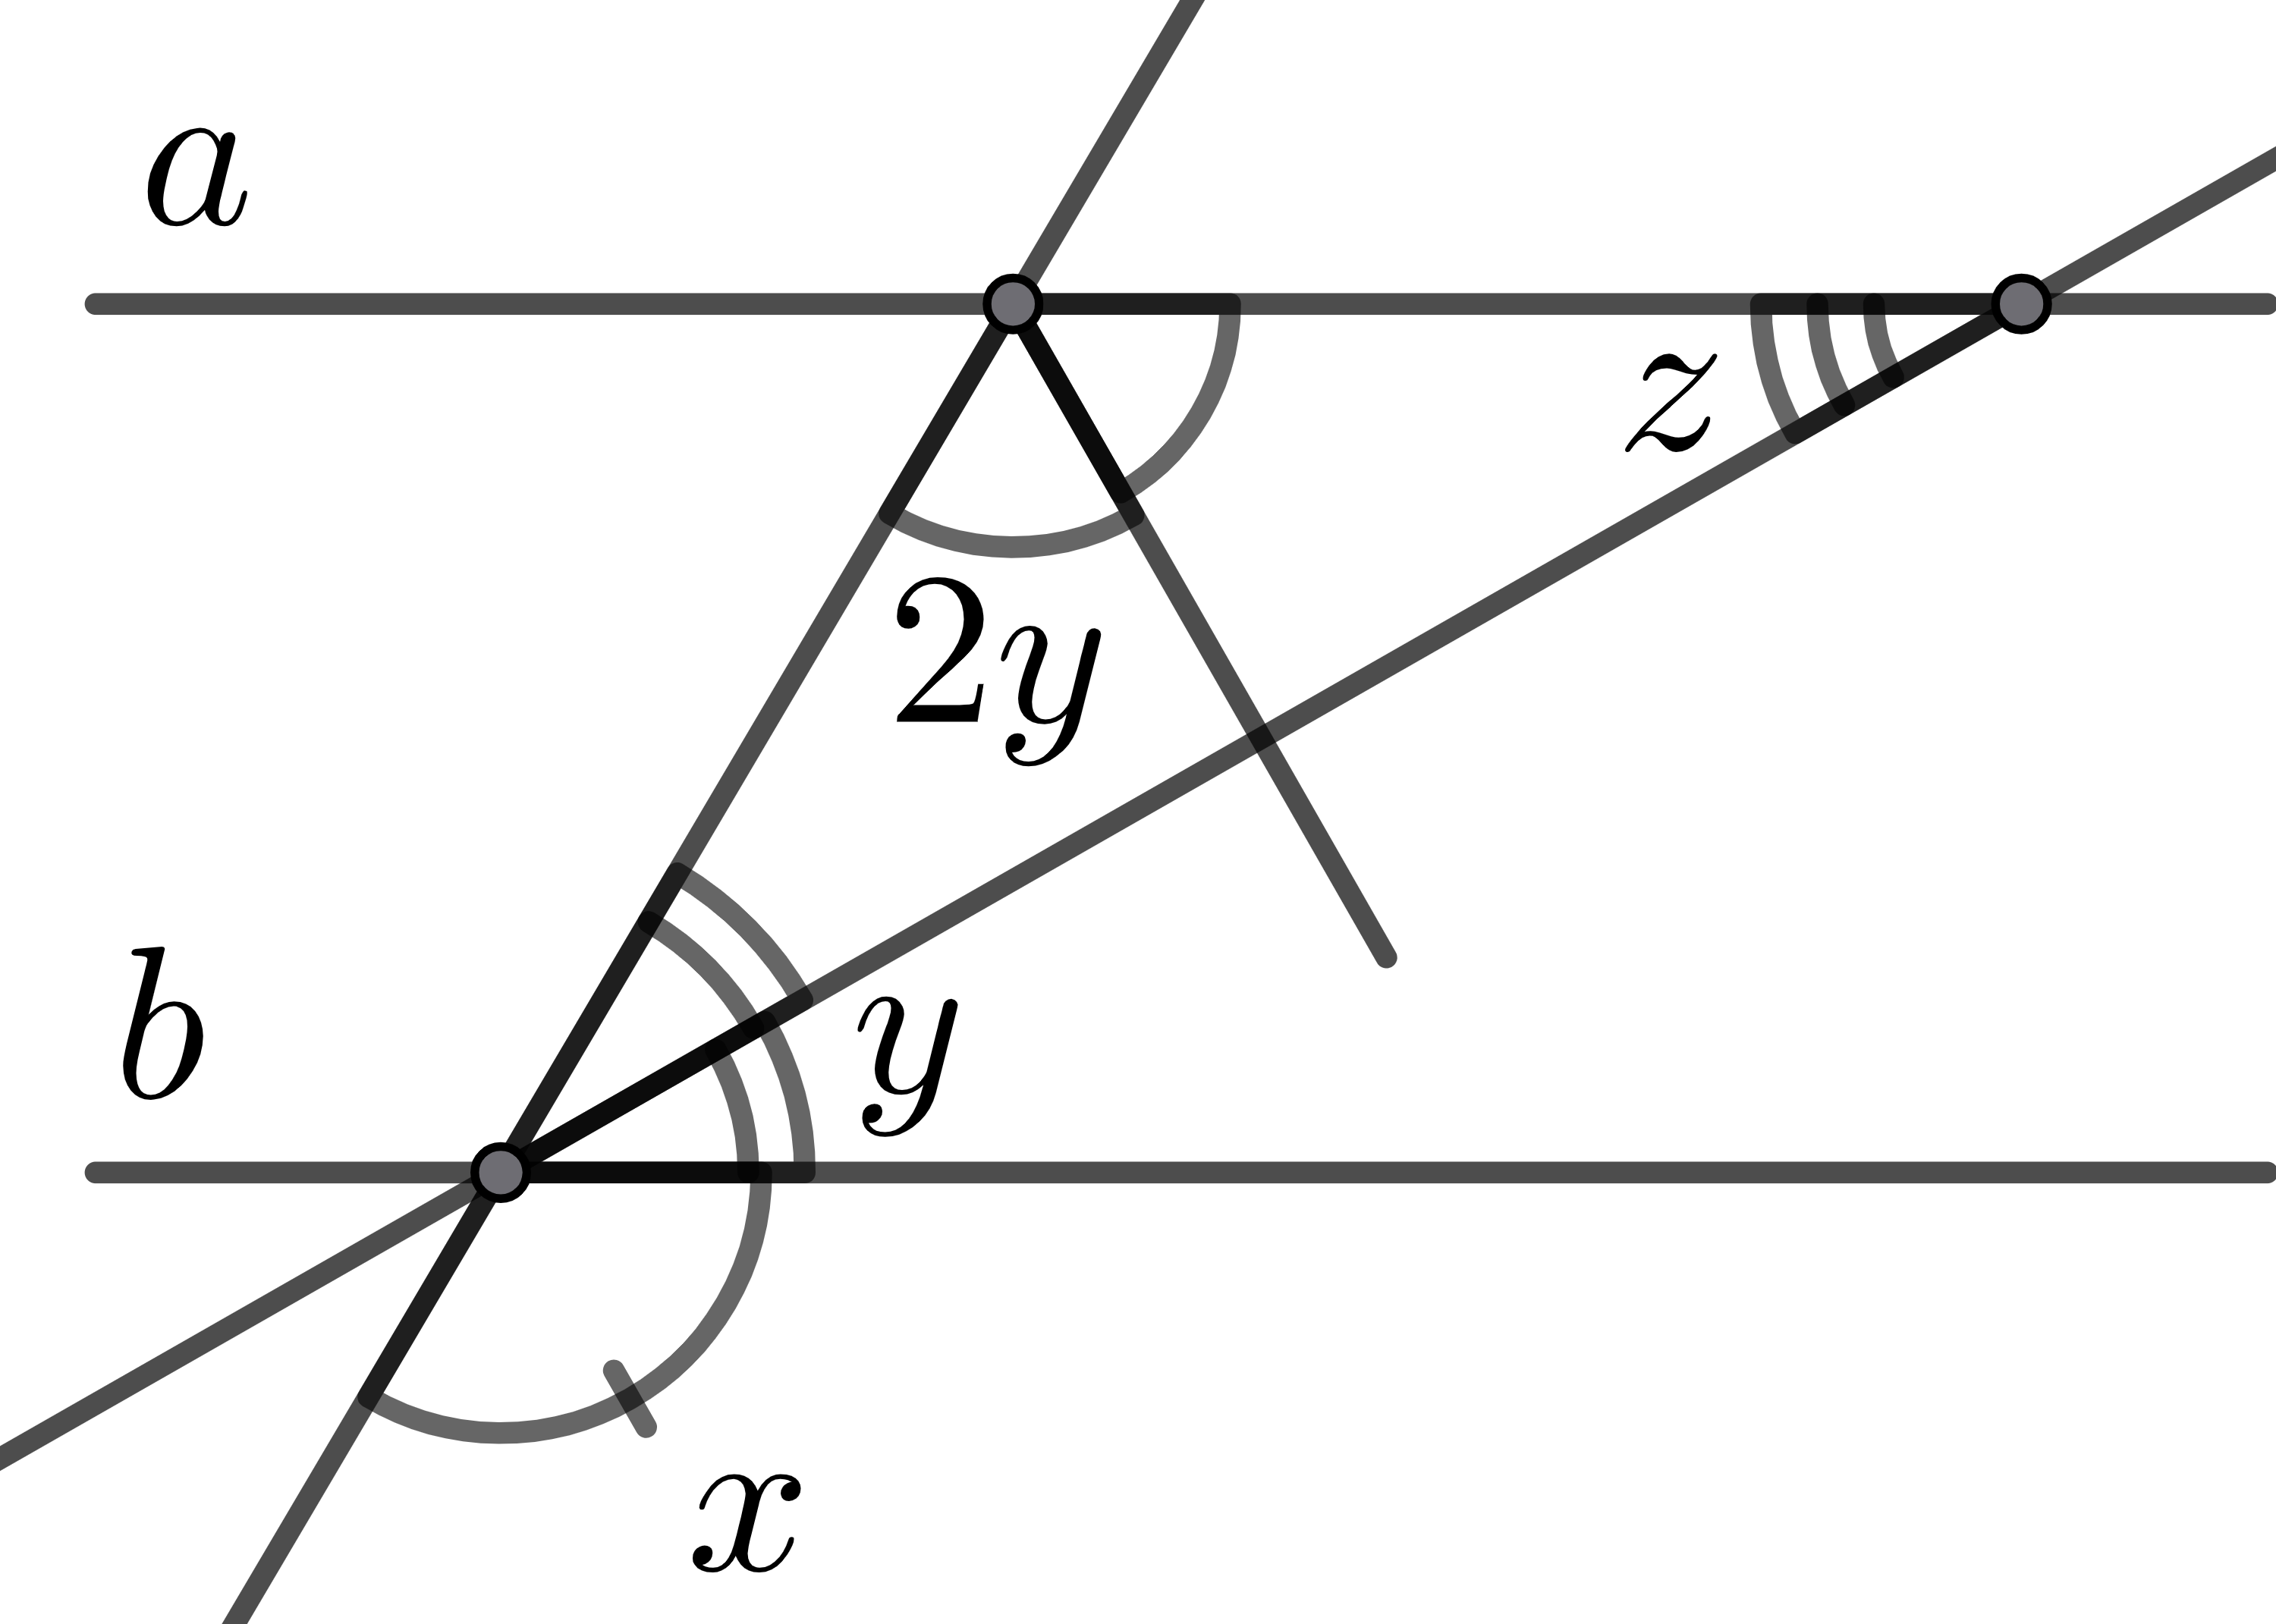
\includegraphics[width=.3\textwidth]{20260404/pics/20260404_geom_for_mat_02b_v2.png}

\samerowans{\begin{problem}{3}
Через точку пересечения биссектрис $\triangle{ABC}$ проведена прямая, параллельная прямой $AC$, пересекающая стороны $AB$ и $BC$ в точках $M$ и $N$ соответственно. $MN=10$, $NC$ на 2 больше $MA$. Найдите длину $MA$.
\end{problem}} 

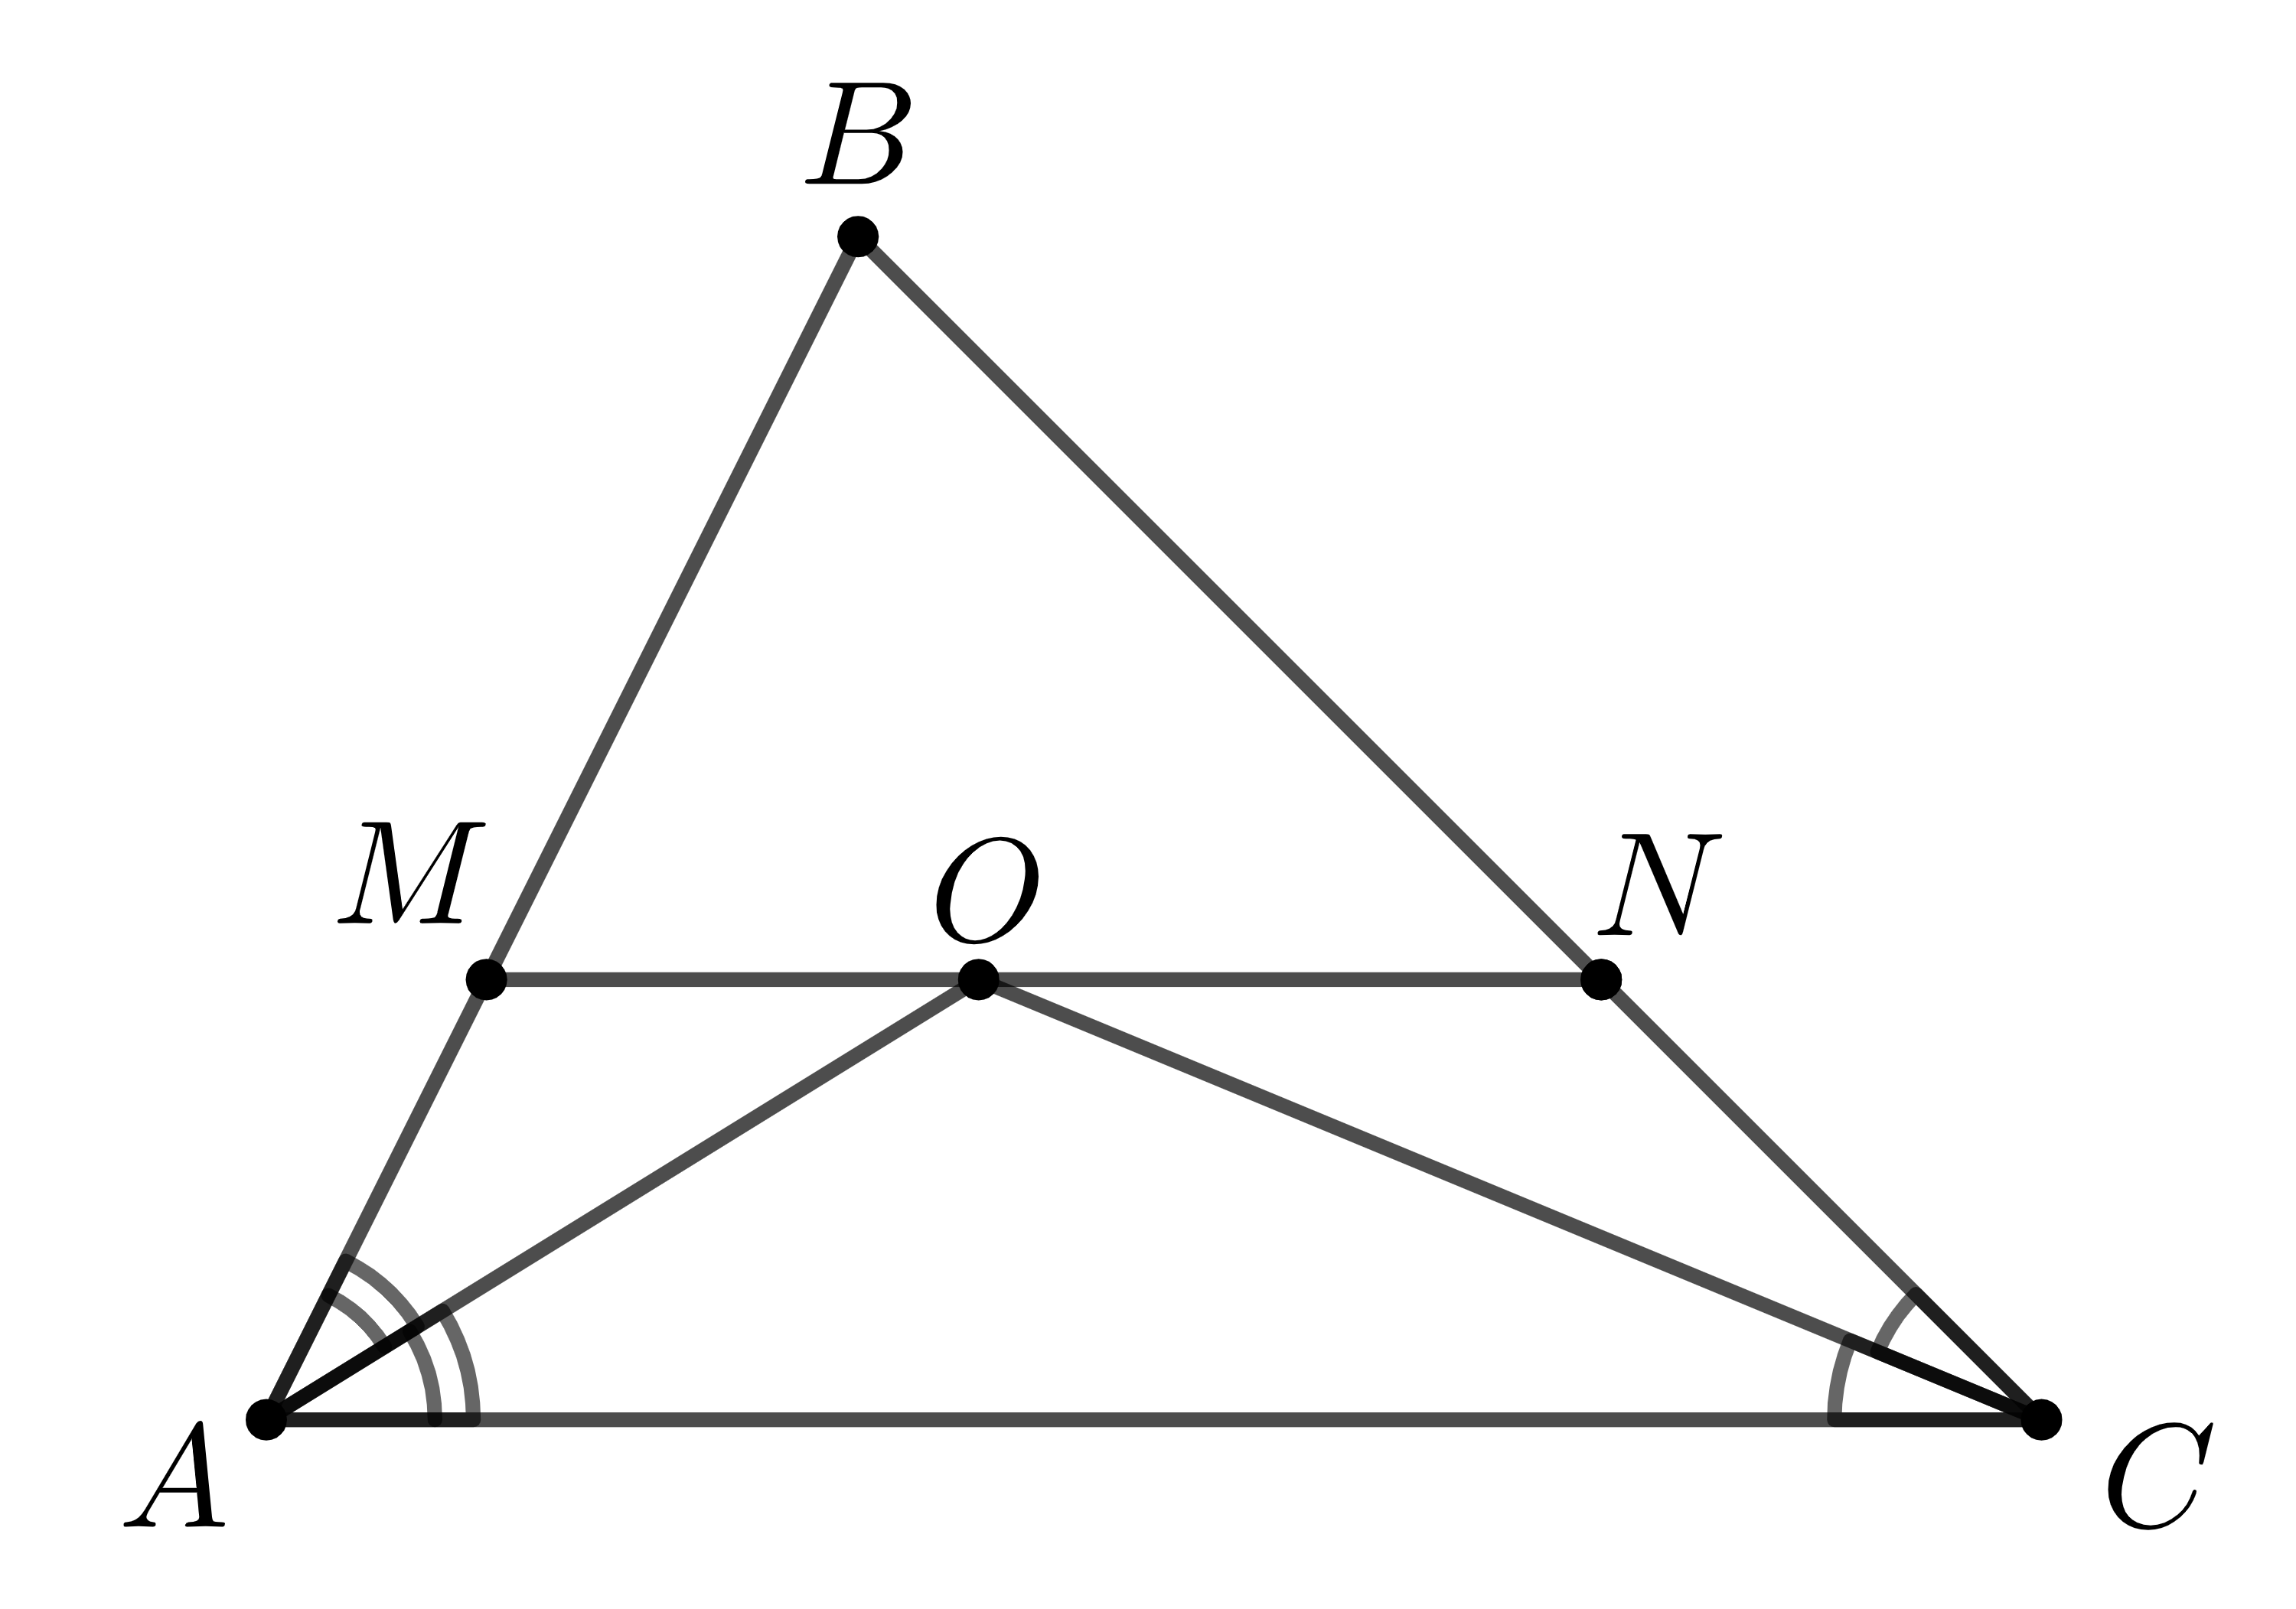
\includegraphics[width=.3\textwidth]{20260404/pics/20260404_geom_for_mat_03_v2.png}

\samerowans{\begin{problem}{4}
Дан равносторонний $\triangle{ABC}$. На стороне $AC$ взята точка $M$ такая, что сумма периметров треугольников $ABM$ и $MBC$ равна 38 см. Найдите длину $MB$, если длина стороны $\triangle{ABC}$ равна 12 см.
\end{problem}} 

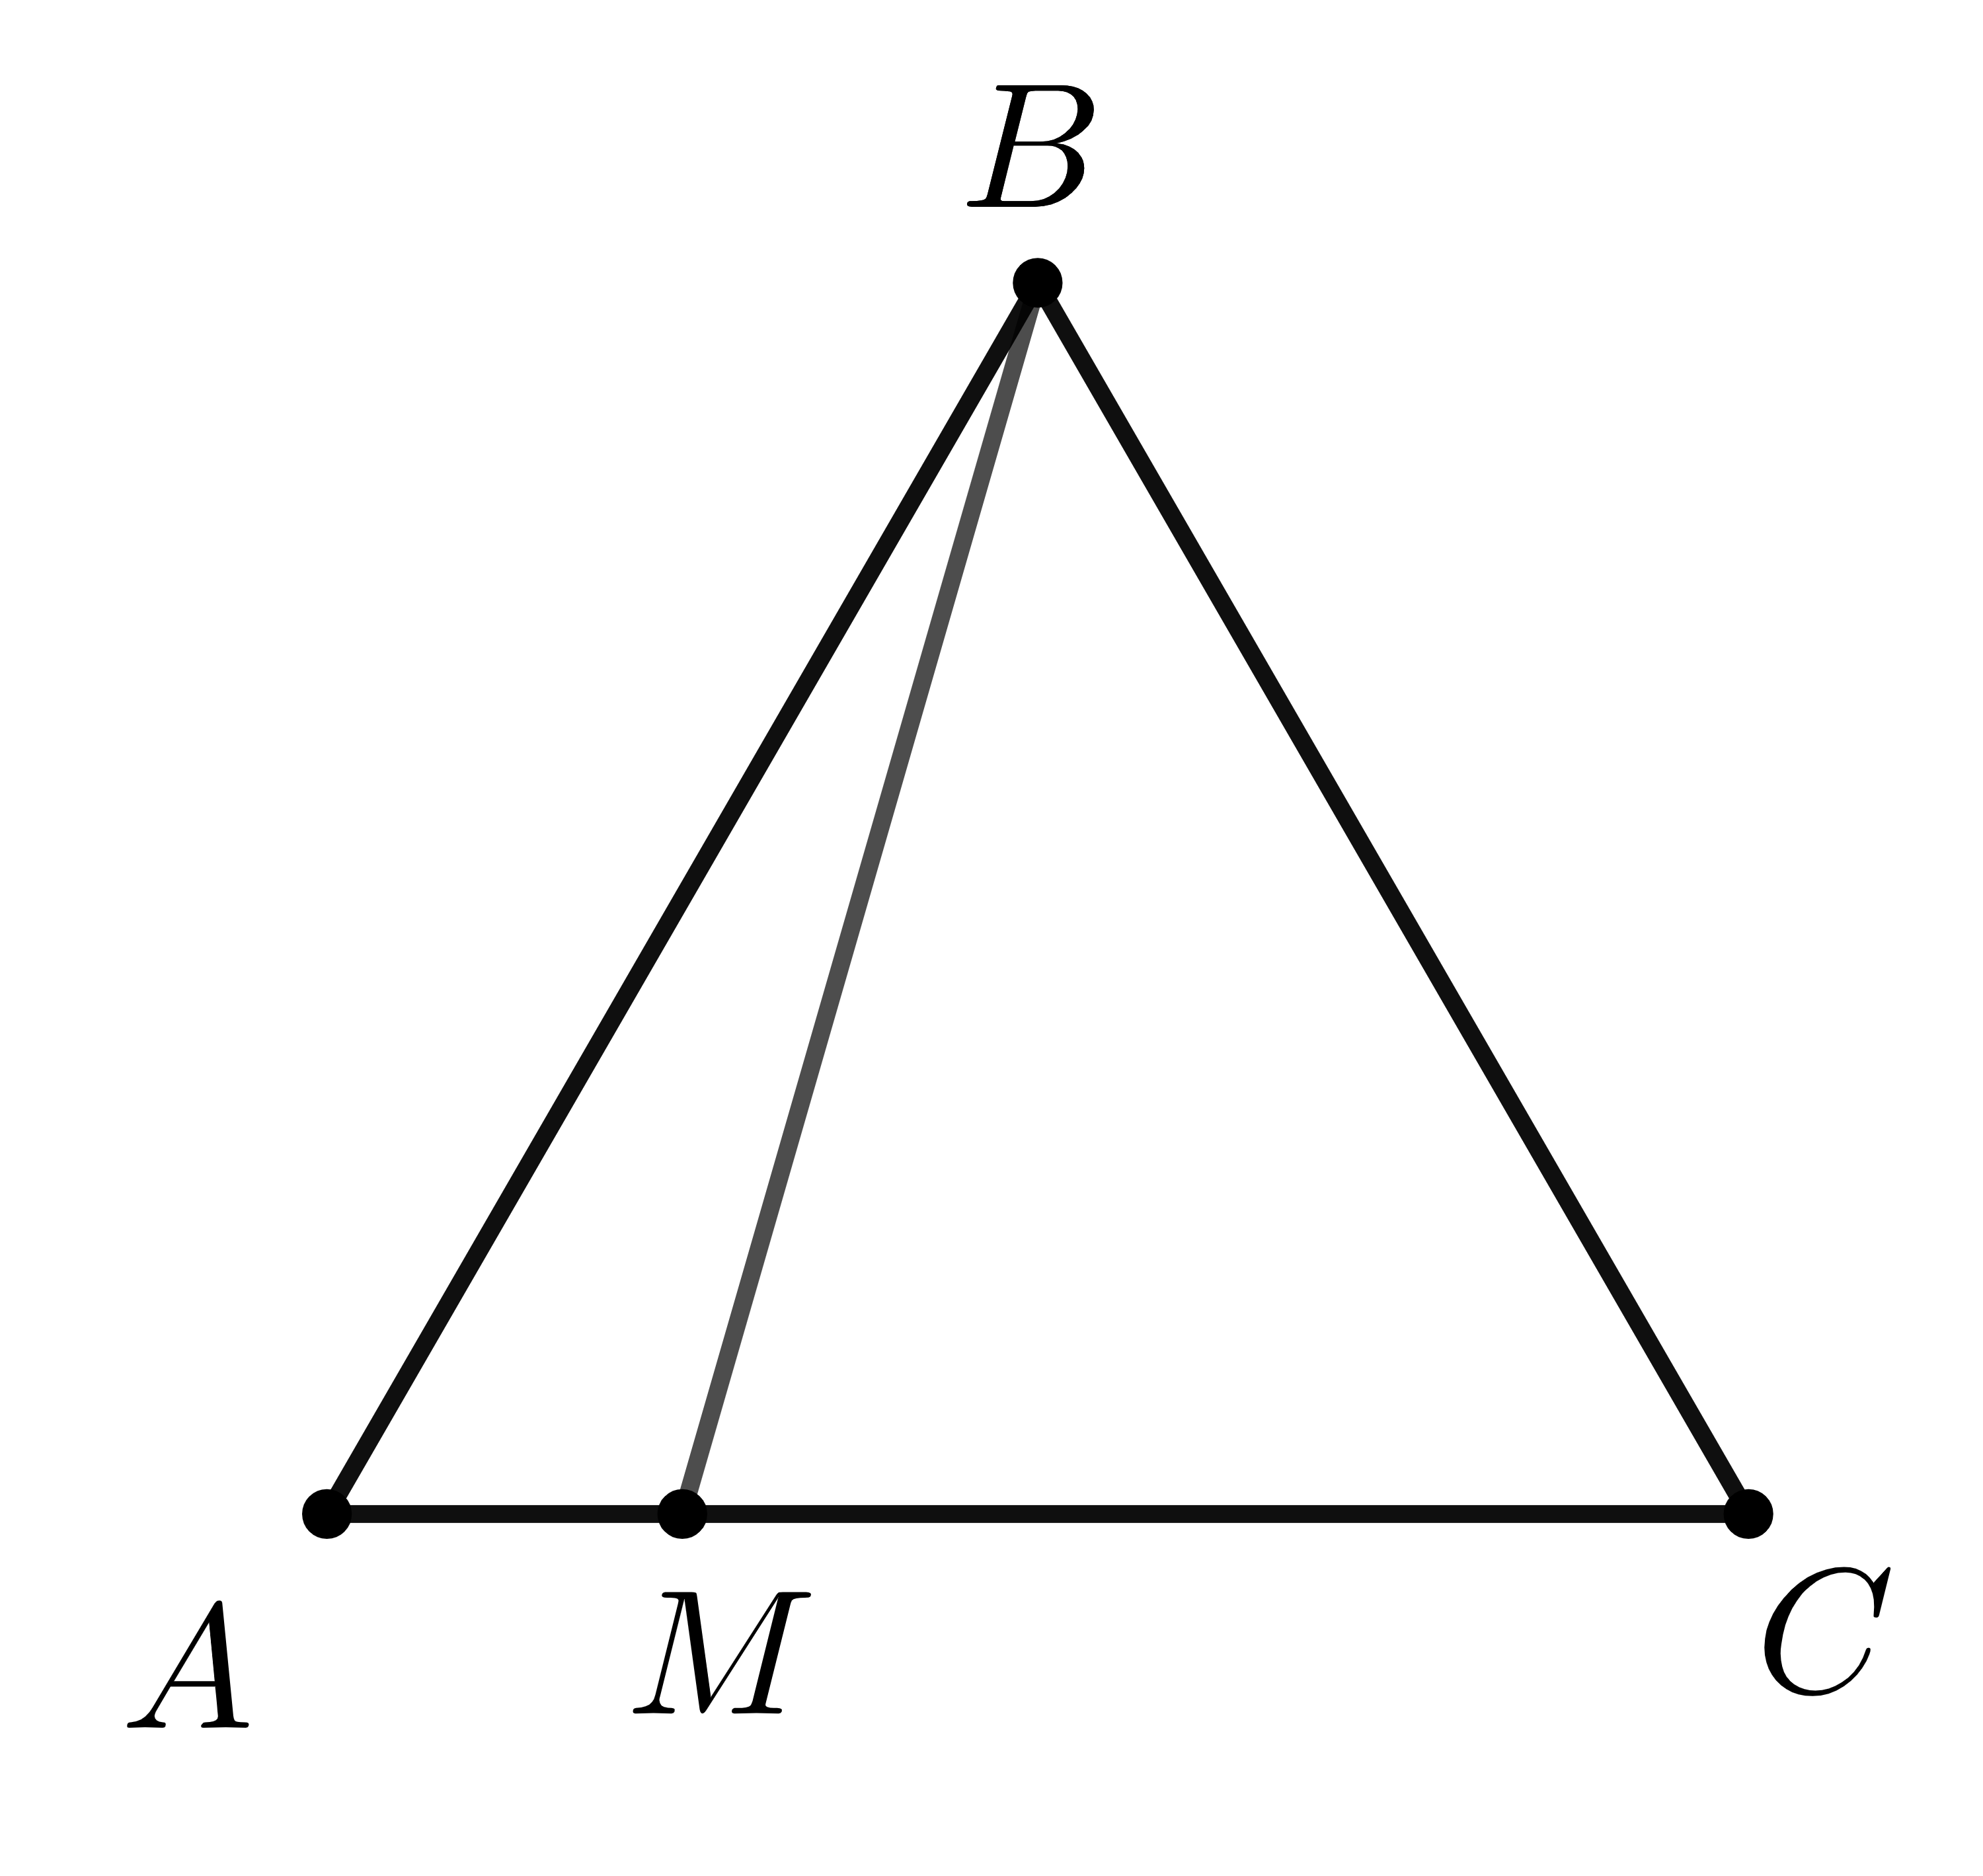
\includegraphics[width=.3\textwidth]{20260404/pics/20260404_geom_for_mat_04_v2.png}

\samerowans{\begin{problem}{5}
Точка $P_1$ --- середина отрезка $CD$. Точка $P_2$ --- середина отрезка $P_1C$. Точка $P_3$ --- середина отрезка $P_2C$. Точка $P_4$ --- середина отрезка $P_3C$. Длина отрезка $P_1P_4=35$ см. Найдите длину отрезка $CD$. 
\end{problem}} 

\samerowans{\begin{problem}{6}
Выпишите номера верных утверждений. Если верных нет --- напишите 0.
\end{problem}}

1) Если сумма двух сторон и периметр одного треугольника равны сумме двух сторон и периметру другого треугольника, то эти треугольники равны. 

2) Если стороны углов соответственно перпендикулярны, то углы равны.

3) Высота остроугольного треугольника не может равняться соседней стороне.

4) Существует прямая, которая параллельна каждой из двух пересекающихся прямых.
 

\samerowans{\begin{problem}{7}
Известно, что $\angle{A} = 36^{\text{o}}$, $\angle{B} = 38^{\text{o}}$, $\angle{C} = 41^{\text{o}}$, $\angle{D} = 46^{\text{o}}$. Найдите $\angle{E}$.
\end{problem}} 

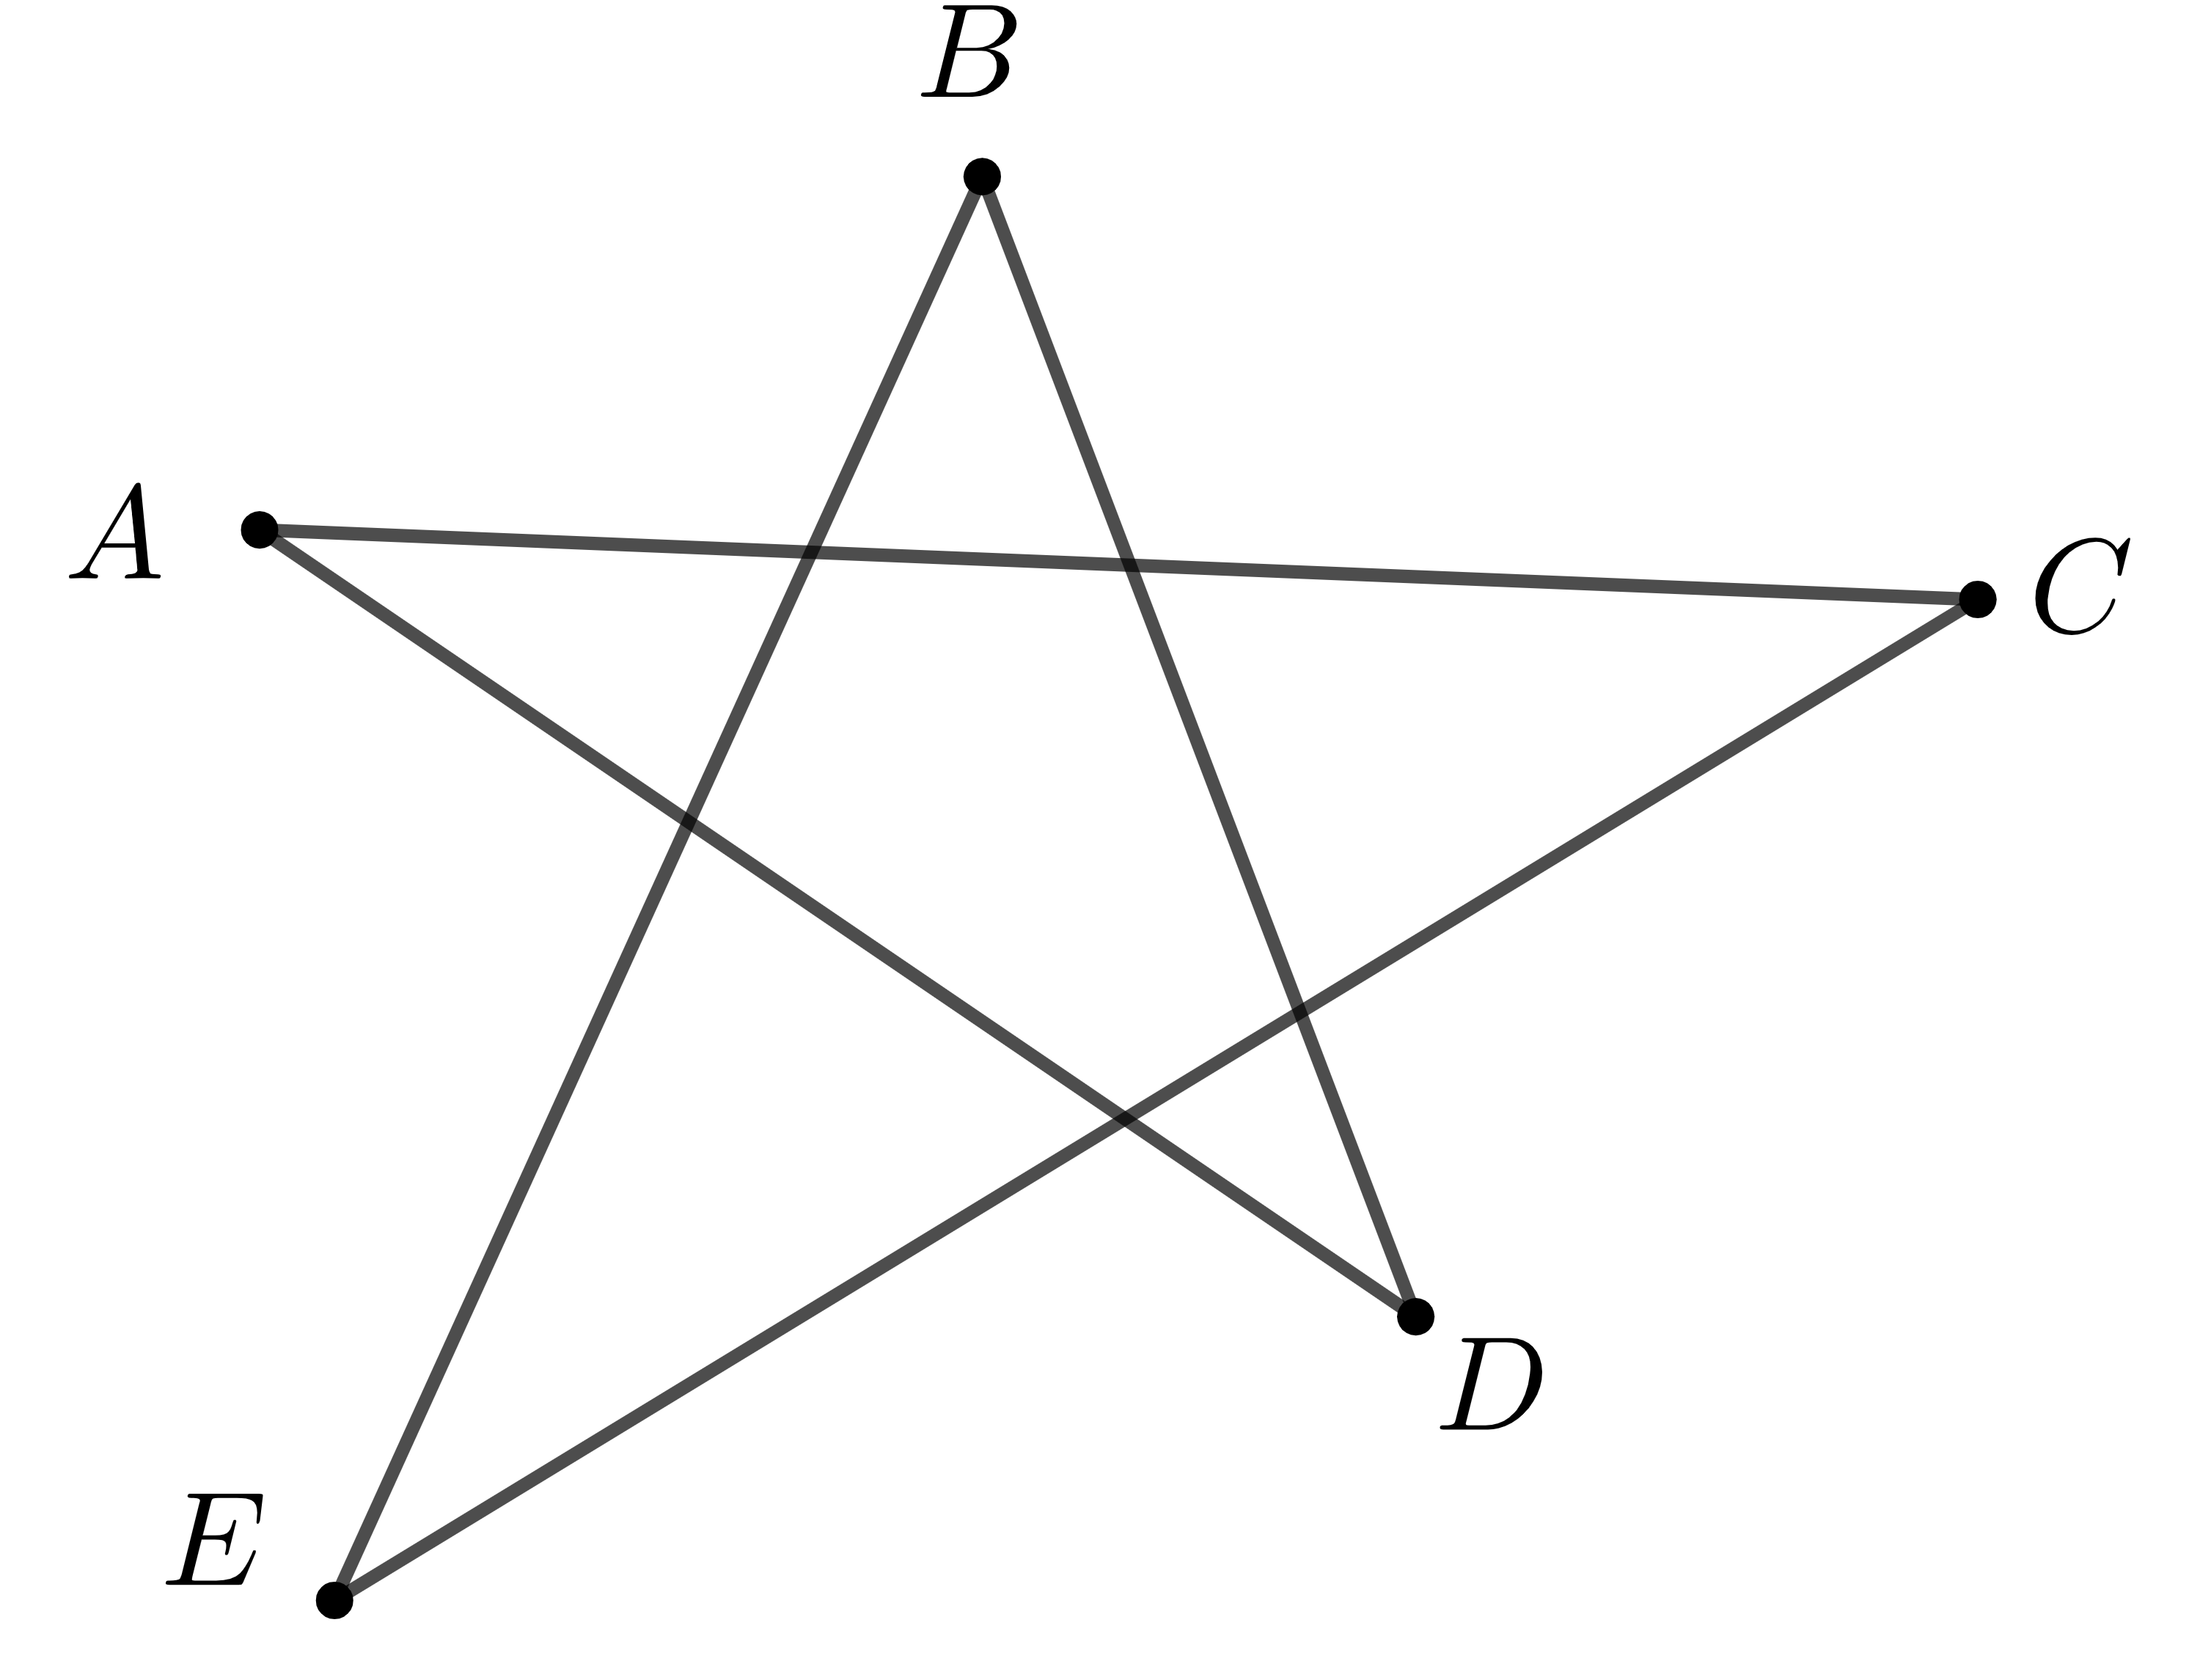
\includegraphics[width=.3\textwidth]{20260404/pics/20260404_geom_for_mat_07.png}

\begin{problem}{8}
На рисунке $BK\perp AC$, $\angle{MBA}=30^{\text{o}}$. Найдите $\angle{NBC}$.
\end{problem}

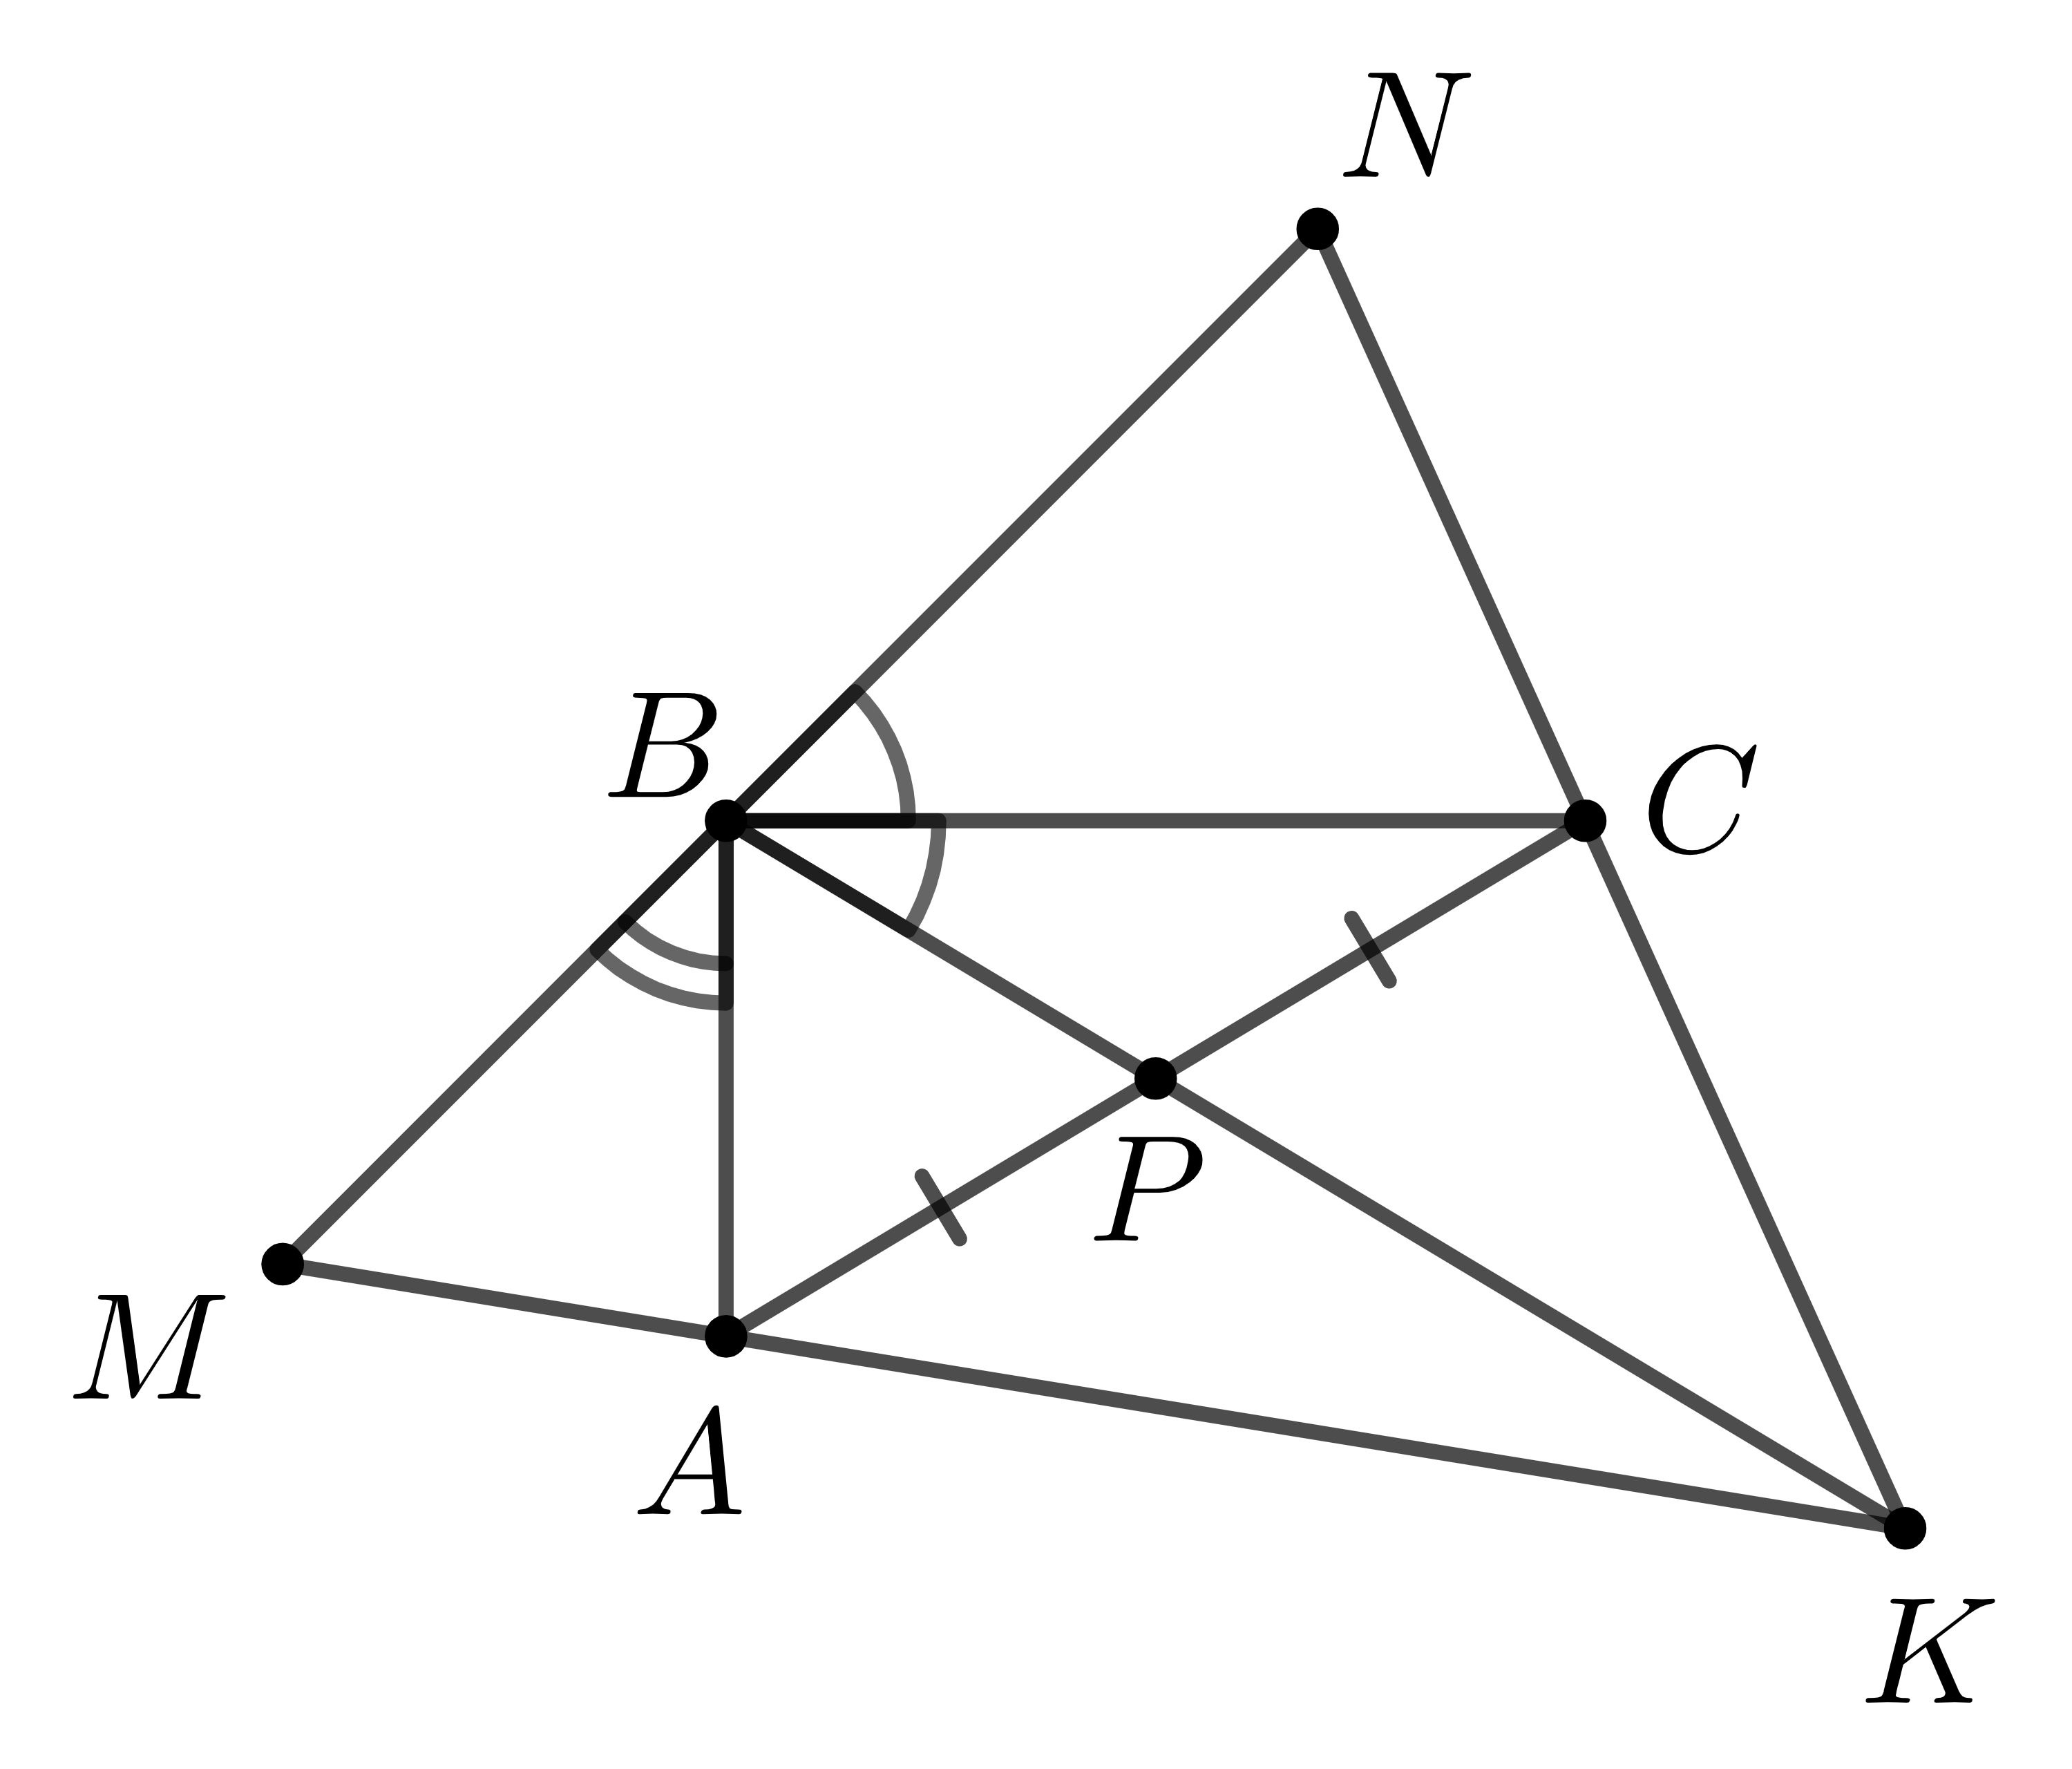
\includegraphics[width=.3\textwidth]{20260404/pics/20260404_geom_for_mat_08.png}

\begin{problem}{9}
Дан четырёхугольник $ABCD$. Известно, что $AC=AD$, $\angle{ABD}=\angle{CBD}=30^{\text{o}}$, $\angle{CAB}=60^{\text{o}}$. Найдите $\angle{CDA}$.
\end{problem}

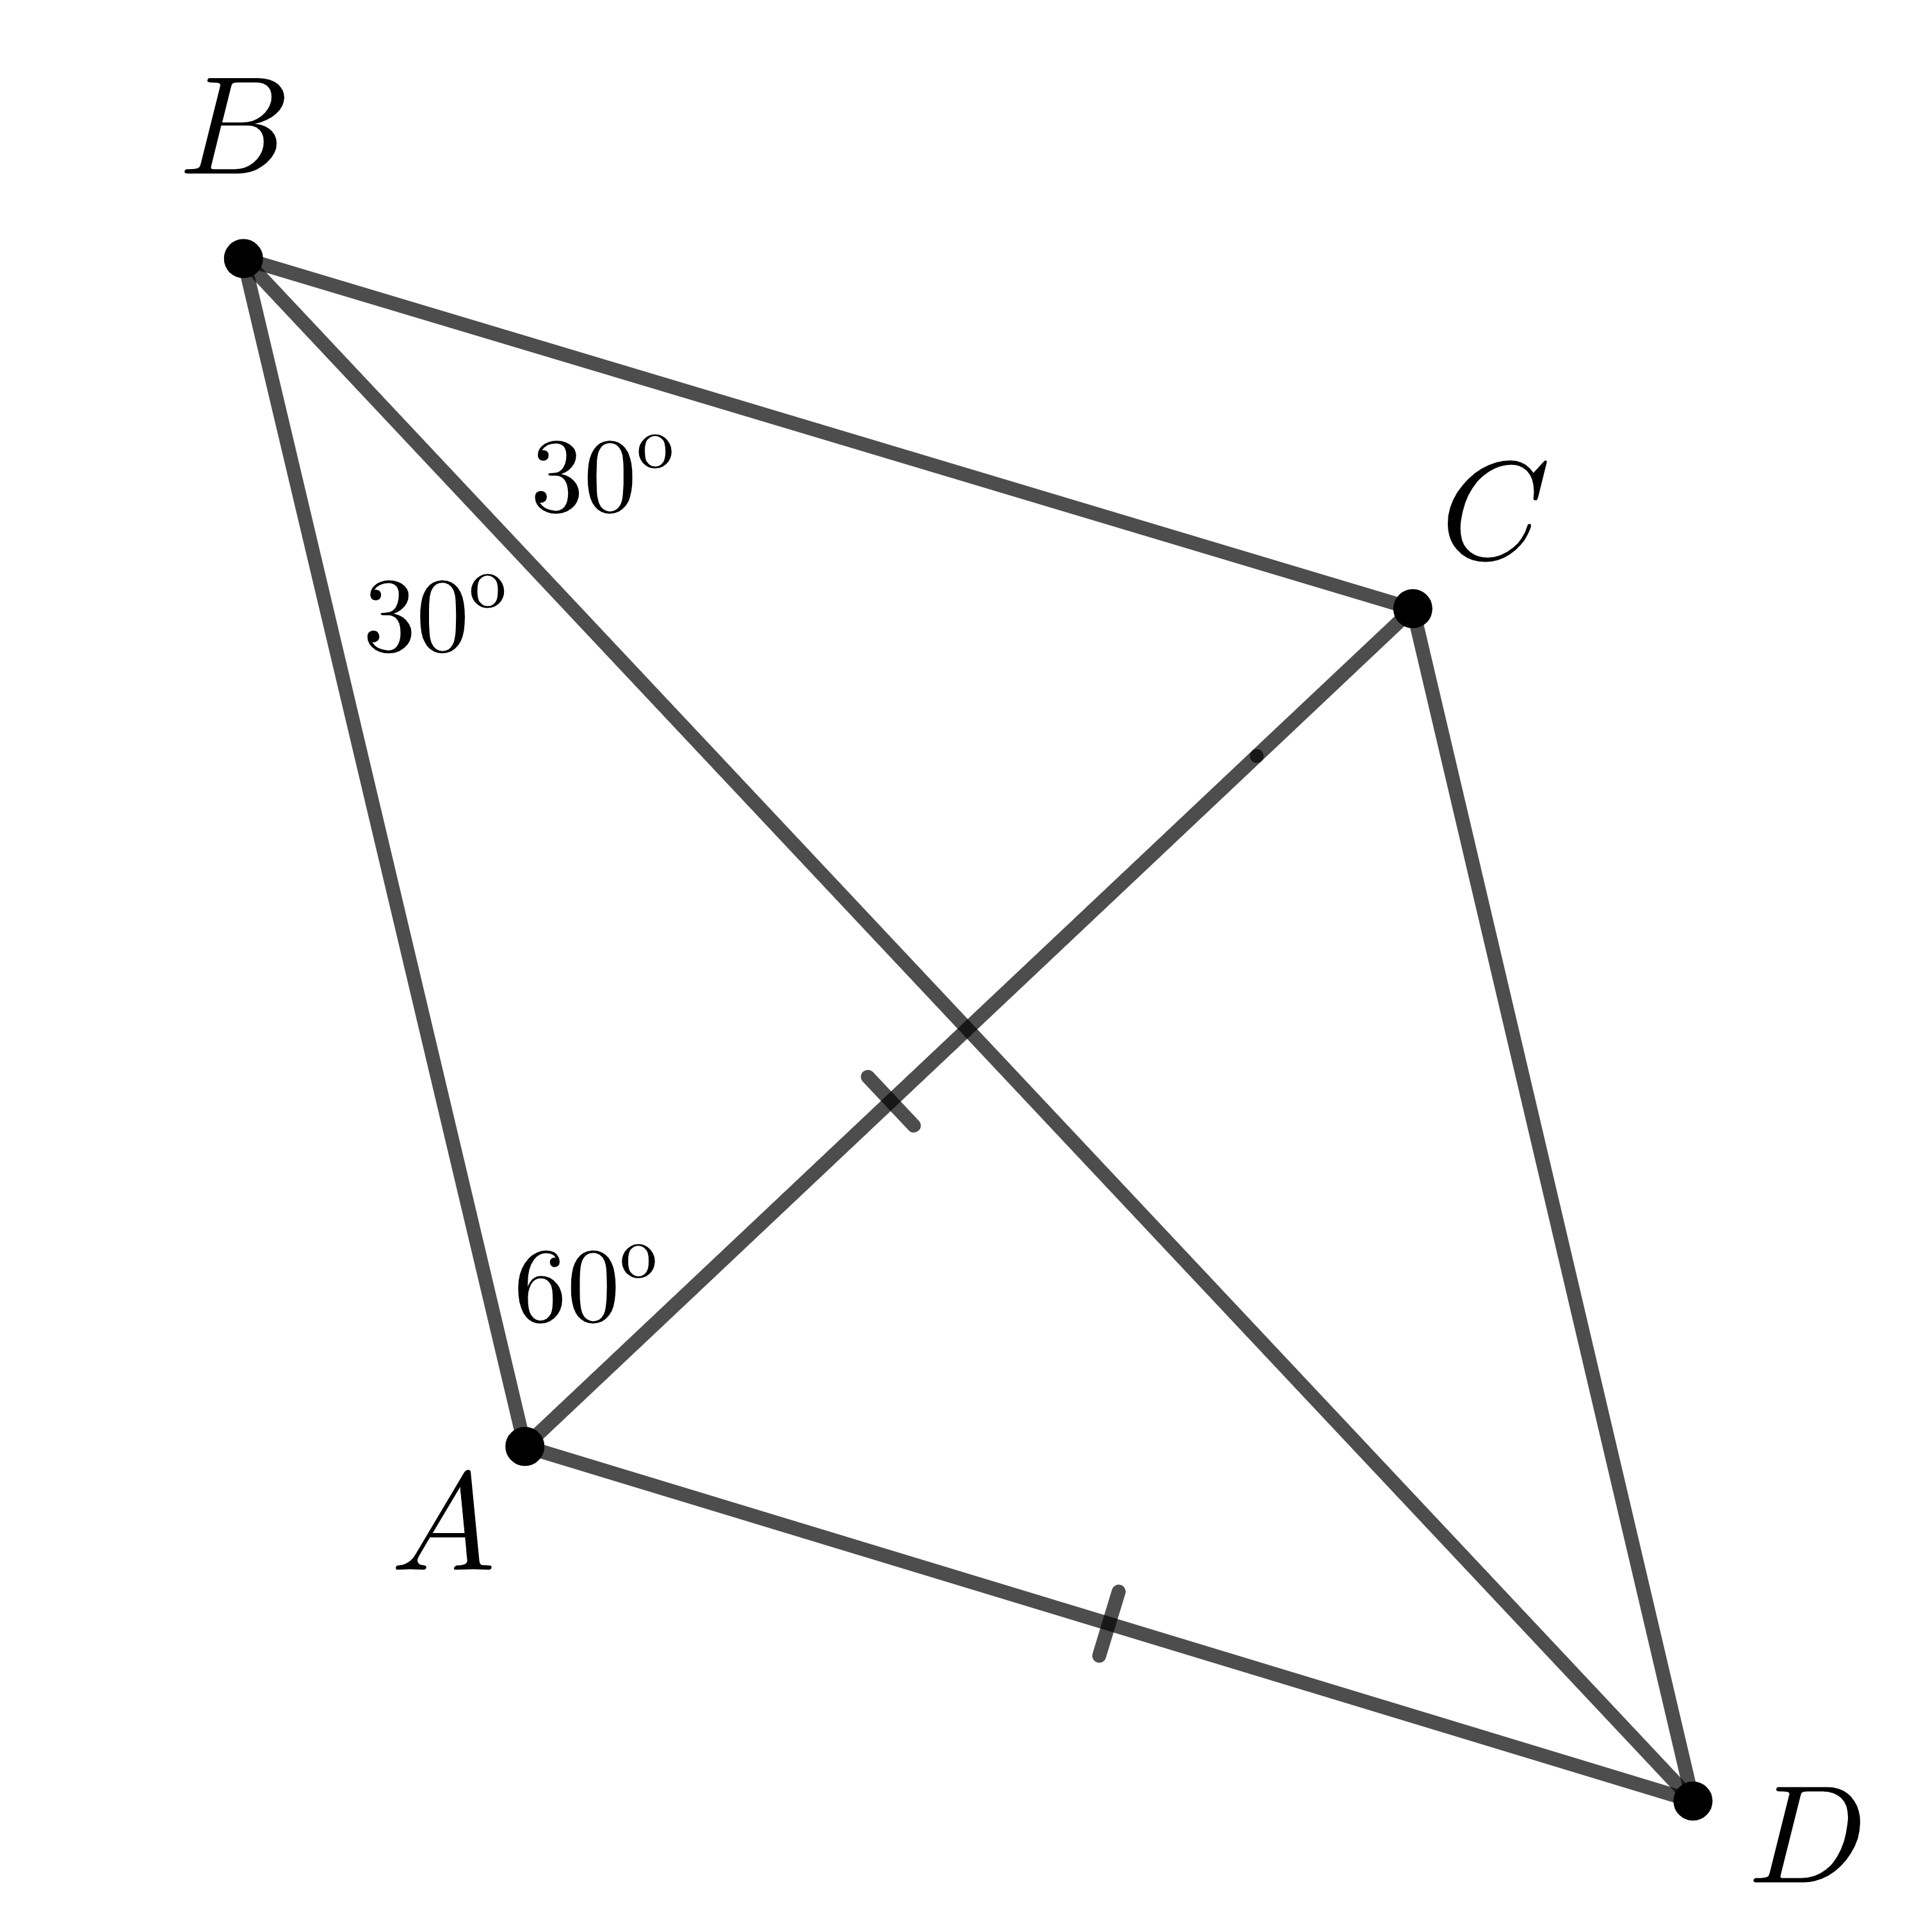
\includegraphics[width=.3\textwidth]{20260404/pics/20260404_geom_for_mat_09_v2.png}

\begin{problem}{10}
На сторонах $BC$ и $CD$ квадрата $ABCD$ взяли точки $K$ и $M$ так, что $BK+DM=MK$.  Докажите, что угол  $MAK$ равен $45^{\text{o}}$.
\end{problem}